\section{\hei{循环分割工具}}
\par{简介:循环分割工具,主要功能,将函数中出现的符合分割条件的for循环,分割出来,当作函数调用来处理.例如:}

\begin{lstlisting}
int main(){
    int i;
    int sum = 0;
    for(i=0;i<100;i++){
        sum += i;
    }
    return sum;
}
\end{lstlisting}

\par{替换后:}
\begin{lstlisting}
int main(){
    int i;
    int sum = 0;
    main_loop_1(i,sum);

    return sum;  
}

void main_loop_1(int *i,int *sum){
    for(*i = 0; *i < 100; *i++){
        *sum += *i;
    }
}
\end{lstlisting}

\par{分割分为两个部分,第一部分收集所需要的信息,如for,参数等.第二部分将收集到的信息写入相应的文件,包含三个文件,source.c newsource.c newheader.h . }
\subsection{\hei{收集信息}}

\par{收集for循环:找到顶层循环并收集到TopLevelLoop中,寻找的策略:从顶节点出发,找到每个函数,然后通过Traverse(FunctionDecl *FD),查找for循环,并且用ForStmtAction规定查找的方式,ForStmtAction = 1时,遍历到for停止,ForStmtAction = 2 时继续遍历.}
\begin{lstlisting}
bool TraverseForStmt(ForStmt *s)
{
    if (!WalkUpFromForStmt(s))
        return false;
    //到达ForStmt节点时,继续遍历.
    if (ForStmtAction == 2){
        for(Stmt::child_range range = s->children(); range; ++range)
            TraverseStmt(*range);
    }
    //到达ForStmt节点时,停止,得到顶层的循环.
    if(ForStmtAction == 1){
        TopLoop.push_back(s);
        //s->dumpColor();
        return true;
    }
    return true;
}
\end{lstlisting}

\par{循环分割条件:循环分割小于指定次数时不分隔,目前只能判断常量的情况,TODO:之后判断变量的情况.下面收集的信息都是针对可以分割的循环进行 的}

\par{收集for的位置信息:存放在LoopPosition中,这样可以从源文件获取和删除for,并替换为调用函数.}

\par{保守性处理:1.循环中调用了本文件中的函数,目前不分割(TODO:可以分割,在头文件中写函数声明),2.用到了在本函数中定义的结构体,不分割(实际情况很少)).}

\par{收集输入参数:存放在llvm::DenseMap<ForStmt*, std::vector<ValueDecl*> > InputArgs,输入和输出的参数一样.策略:遍历ForStmt,收集到在循环中定义的和使用的函数,使用的去掉定义的,若为全局变量的话,也不作为参数,这样得到要传入的参数.其中对于sizeof(a),a是个数组时,当做参数传入时,只会作为指针传入,这是要找到数组的大小变量 n或者是一个常量100或是宏;若是变量时,也当作参数传入,此时循环中的sizeof(a)替换为sizeof(元素类型)*(*n),或 sizeof(元素类型)*100.}


\par{收集调用模板和函数声明模板:存放在CallProto和FunctionProto中.策略:CallProto = 函数名 + 参数列表 + ";",函数名 = FDName + \_loop\_ + number,参数列表可以通过前面的得到的输入参数构造. 函数模板声明的构造方式一样,参数作为指针传入 (如 int *i),)  }

\par{收集循环的内容和构造调用的函数:通过LoopPosition中的位置信息,由接口getForStmt获取循环的内容,并根据收集到的参数,把循环中对应的变量做替换,因为传入的时候用的指针,替换成(*VarName),结合函数声明模板,得到调用的函数,调用的函数如下.对于引用中的与参数名字相同的字符串不替换,收集到成对 " 的位置,在一对中间的话不替换, 具体的实施方法参考代码.}
\begin{lstlisting}

FunctionProto {
    替换后的LoopContent
}
\end{lstlisting}

\par{若循环中出现 return,如return a+b 或 return ; 带用返回值这根据返回值的类型确定调用的函数返回值的类型,并增加一个参数 re,传递a+b的值,循环中的return a+b;替换成(*re) = a+b; 源文件中也要做相应的改动,例如增加 int re = CallProto;return re;语句来替换循环.  }

\begin{lstlisting}
    //源代码
    for(i = 0 ; i<100;i++){
        if(i==50) return sum;
    }
    //替换后的源代码
    { int re_arg_pa1_2 = -1; int re_arg_pa2_2;
    
     main_loop_2(&i, &sum, &re_arg_pa1_2, &re_arg_pa2_2);
        
     if(re_arg_pa1_2 != -1) return re_arg_pa2_2; }

    //新的源代码

    for((*i) = 0 ; (*i)<100;(*i)++){
        if((*i)==50) { (*re_arg_pa1_2) = 0; (*re_arg_pa2_2) = (*sum); return; }
    }

\end{lstlisting}

\par{收集要写入头文件的信息,通过接口getHeader(),目前的做法是将文件头部的信息,如"\#include.."和注释放到头文件中}

\subsection{\hei{写文件}}


\par{写三个文件,源文件,新的.c文件,头文件.命名规则:新的.c文件名 = 原文件名 + \_loop\_ + for循环数目 +.c,头文件与新的.c文件名相同,后缀为.h 例如:test.c,分割出来两个循环,新文件名test\_loop\_2.c,头文件test\_loop\_2.h .}

\par{test.c:先将\#inclule "test\_loop\_2.h"写入到test.c中,之后写入其他的内容,目前的做法是将结构体提取到头文件中,在test.c中不包含结构体的声明,在将函数中相应的for循环替换为调用函数.}

\par{test\_loop\_2.c:先包含\#include "test\_loop\_2.h",写入到相应宏的信息,(TODO:变量声明的话,可以extern声明,例如:extern int a; )之后将收集到循环对应的函数写到文件中.}

\par{test\_loop\_2.h:目前的做法,头文件中,包涵原文件文件头部,结构体声明,之后将收集到的函数模板生命放到头文件中}


\subsection{\hei{问题}}
\begin{itemize}

\item{\hei{利用位置信息提取原代码}}

\par{开始在数组LoopPosition存放的是循环的起始行和结束行的信息,通过起始行和结束行得到循环的代码,但是在测试中发现,在结束行有时会存在注释从结束行开始,并延续到后面几行,之后是想通过行列信息提取,在得到的行列信息出新的情况如下:}

\begin{lstlisting}
//LoopExtractor.cpp的代码
....
SourceManager &SM = context.getSourceManager();
int lineStart = SM.getPresumedLoc(SR->getBegin()).getLine();
int lineEnd = SM.getPresumedLoc(SR->getEnd()).getLine();
int colStart = SM.getPresumedLoc(SR->getBegin()).getColumn();
int colEnd = SM.getPresumedLoc(SR->getEnd()).getColumn();
...
llvm::outs() << "For:" << lineStart << "  " << colStart << "  " << lineEnd << "  " << colEnd << " \n";
....

//测试例中的代码

44 
45 for(i = 0 ; i<100;i++)
46 sum++;
47

//结果:如图1
        
//对于以下的代码
44 
45 for(i = 0 ; i<100;i++)
46 {sum++;}
47 
        
//结果图2:
                
For:45  1  46  8 
                
\end{lstlisting}


\begin{figure}
\centering
\includegraphics[width=3in,height=0.5in]{img/forLocationResult0.png}
\caption{location1}
\label{forLoactionResult0}
\end{figure}

\begin{figure}
\centering
\includegraphics[width=3in,height=0.5in]{img/forLocationResult.png}
\caption{location2}
\label{forLoactionResult}
\end{figure}

\par{由于给出的位置信息分号没有算进去,现在的做法:在结束行,找到最后一个"/*",提取前面的部分.}

\item{关于宏的问题}

\par{在预处理阶段,处理并保留的宏的相关信息,每个宏的信息保存在了相应的类MacroInfo 中,从CompilerInstance \&CI的到类preProcessor,通过其中的迭代器macro\_begin(),迭代访问每一宏的信息,并保存在MacroInFile,MacroContentInFile等数组中,为后的处理提供信息.}

\par{现在可以将在预处理收集到的宏,写入到新的.c文件中,写的方法:}
\begin{lstlisting}
//加入源文件中有 #define N 100
//写到.c中的代码:

#ifndef N
#define N 100
#endif
\end{lstlisting}
\par{对于函数中的宏定义,出现错误,还需继续处理.}

\begin{lstlisting}
# define SUCCESSOR(name) ((name)->next)
.
.
for (cursor = list, counter = first_length - 1;
           counter;
           cursor = SUCCESSOR (cursor), counter--)
    continue;
      second_list = SUCCESSOR (cursor);
        SUCCESSOR (cursor) = 0;
.
.
#define SUCCESSOR
\end{lstlisting}
\par{先前得到MacroInfo,不能找到上述的宏定义,可能通过IdentifierInfo得到的MacroInfo,得到的宏不完全(猜测:一个IdentifierInfo对应的几个macro,从identifierInfo类找MacroInfo找的不准确),查找宏的迭代器typedef llvm::DenseMap<const IdentifierInfo *, MacroDirective*>::const\_iterator macro\_iterator,TODO:不是通过IdentifierInfo找MacroInfo,而是直接MacroDirective类直接获得宏,再由接口MacroDirective *getPrevious(),得到相关的宏.)}
\begin{lstlisting}
#include "stdio.h"
#ifndef NO
#define NO 10
#endif


#define N \
          100
int main(int argc, char **argv) {

#define N1 100
.
.
.
#undef N1
}
//输出结果:
zql@zql:~/desktop/LoopExtractor00$ ./test.sh
N  30  31
NO  5  5
//N1出现问题.

\end{lstlisting}
\item{getHeader()}

\par{先前提取头文件的策略是从文件头部查找,在遇到第一条语句之前,当遇到"\#..."时,放到头文件中,若出现"\#if..."时,查找到"\#endif",对于system.c中代码如图,则将整个文件全部提取到头文件中,出现错误,修改:因为现在增加了宏的查找(TODO:具体还没有完善),则只查找文件头部的\#inclule...语句,}
\begin{lstlisting}
\\system.c中的代码

#include "system_loop_2.h"
#if MSDOS

bool
sys_get_archive_stat (void)
{
  return 0;
}
.
.
.
.
#endif /* not MSDOS */
//文件的尾部
\end{lstlisting}
\par{分割完成后,出现的其他几个未解决问题,经过手工修改后,可以编译通过,但是在链接出现了,为定义的错误,如图.但是在用以前提取头文件的方法程测试,手动修改了几个分割是未识别的问题,能够编译通过.}
\begin{figure}
\centering
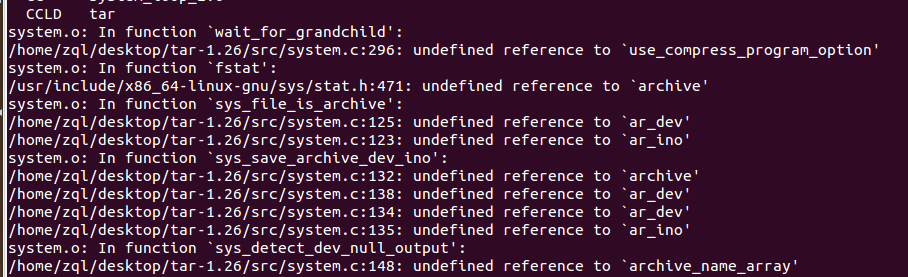
\includegraphics[width=3in,height=1in]{img/tarCCLD.png}
\caption{tarCCLD}
\label{tarCCLD}
\end{figure}


\item{部分变量未识别的问题}
\par{还以以前的buf为例,单独分割时并没有出现,没有问题,当和其他文件一块分割时,buf未分割,相应的sizeof.的问题也出现了,头文件没有包含.将所有的头文件加入后,未出现问题.}

\par{错误1:数组中的宏未定义的错误}
\begin{lstlisting}
buffer.c:
static struct zip_program zip_program[] = {

  { ct_compress, COMPRESS_PROGRAM, "-Z" },
  { ct_compress, GZIP_PROGRAM,     "-z" },
  { ct_gzip,     GZIP_PROGRAM,     "-z" },
  { ct_bzip2,    BZIP2_PROGRAM,    "-j" },
  { ct_bzip2,    "lbzip2",         "-j" },
  { ct_lzip,     LZIP_PROGRAM,     "--lzip" },
  { ct_lzma,     LZMA_PROGRAM,     "--lzma" },
  { ct_lzma,     XZ_PROGRAM,       "-J" },
  { ct_lzop,     LZOP_PROGRAM,     "--lzop" },
  { ct_xz,       XZ_PROGRAM,       "-J" },
  { ct_none }
};

suffix.c:
static struct compression_suffix compression_suffixes[] = {
#define __CAT2__(a,b) a ## b
#define S(s,p) #s, sizeof (#s) - 1, __CAT2__(p,_PROGRAM)
  { S(gz,   GZIP) },
  { S(tgz,  GZIP) },
  { S(taz,  GZIP) },
  { S(Z,    COMPRESS) },
  { S(taZ,  COMPRESS) },
  { S(bz2,  BZIP2) },
  { S(tbz,  BZIP2) },
  { S(tbz2, BZIP2) },
  { S(tz2,  BZIP2) },
  { S(lz,   LZIP) },
  { S(lzma, LZMA) },
  { S(tlz,  LZMA) },
  { S(lzo,  LZOP) },
  { S(xz,   XZ) },
#undef S
#undef __CAT2__
};

\end{lstlisting}
\par{出现未定义错误的这些宏对应的定义都在tar-1.26/config.h中,但在分割时已经包含对应路径,不知道为什么会出现未定义的错误}
\par{错误2:某些变量写入分割后的头文件未写全}

\begin{lstlisting}
suffix.c:

static int nsuffixes = sizeof (compression_suffixes) /
                        sizeof (compression_suffixes[0]);

\end{lstlisting}
\par{nsuffixes变量定义只写进了第一行,第二行未写入的原因可能是因为compression\_suffixes数组中的宏未识别引起的错误}
\end{itemize}
